\documentclass[twoside,twocolumn]{article}
\usepackage[pdftex]{graphicx}
\usepackage[utf8]{inputenc}
\begin{document}
\marginpar



\begin{abstract}


\end{abstract}

\section{Introduction}

Type Ia supernovae (SNe Ia) are known to be the result of a thermonuclear explosion of a C/O white dwarf (WD). A satisfactory description of the progenitor system, however, has yet to be reached. The two most likely configurations for the progenitor systems includes a WD-WD binary, known as the double degenerate (DD) model, or a WD binary with a non-degenerate companion, known as the single degenerate (SD) model. Very early observations (2-3 weeks pre B band maximum) of SNe Ia can show signatures of ejecta interaction with the companion star, and thus can be helpful in determining properties of the progenitor system. However, because the angle at which we observe the SNe Ia restricts the possibility of detecting this emission, <10 of SNe Ia are expected to show signature of this ejecta interaction (Kasen et al 2010).
    
    Through the Phillips relation (Phillips et al 1993), SNe Ia have been used as standard candles to gauge cosmological distances. However, this assumes SNe Ia can be described as a one parameter family. It has recently become more clear that the spectral and photometric features of SNe Ia are diverse, especially at early times. Understanding the relationship between the different spectroscopic and photometric features can help improve our use of SNe Ia as cosmological distance probes, as well as uncover new ideas about the progenitor systems.
    
In this paper, we analyze early observations of SNe Ia iPTF16hvw, discovered by the intermediate Palomar Transient Factory. 
 
\section{Data}
\section{Optical Spectra}
We obtained four optical spectra of iPTF16hvw. These observations were obtained between -16.5 and +13.5 days with respect to B band maximum. (Information on telescopes and instruments)

Using the SN classification software GEneric cLAssification Tool (GELATO) (Harutyunyan et al.), SN 2002dj and SN 2002bo were identified as close spectral matches to the iPTF 16hvw spectra obtained at +5.5 and +13.5 d. Figure 1 shows a spectral sequence including our 4 observations of iPTF16hvw, as well as comparison spectra of SN 2011fe, SN 2002dj and SN 2002bo (Pignata et al 2008; Benetti et al 2004; Blondin et al 2012; Pereira et al 2013; Matheson et al 2008; Aldering et al 2002). At phase +5.5 d, it is clear the Si II $\lambda 6355$ and the Ca IR triplet absorption features in iPTF16hvw are much deeper and broader than in SN 2011fe. At +8.0 days, the spectra for SN2002dj is almost identical to the spectra of iPTF16hvw at +5.5 days, and at +13.23 days, SN2002bo is nearly identical to iPTF16hvw at +13.5. 

To model the Si $\lambda 6355 $ and Si $\lambda 5972$ absorption features we fitted Gaussian kernels, as well as a linear term to account for the continuum. By integrating the Gaussians we obtained equivalent width measurements at +5.5 d, the spectra closest to maximum light, of 136.84 and 18.34 Angstroms respectively. In the Branch classification scheme of SNe Ia (Branch et al 2006), these measurements classify iPTF16hvw, like SN2002dj and SN2002bo, as a broad line SN (Branch et al Fig. 1).  

Absorption velocities were measured using the centroid of the Gaussian fits at -16.5, +5.5 and +13.5 days for the Si II $\lambda 6355 $ and Si II $\lambda 5972$ lines. The relatively high Si II $\lambda 6355 $ velocities are consistent with the broad line classification (Miller et al Fig 3.). However, the Si $\lambda 5972$ line suffered from line blending at +13.5 days, leading to an inaccurate velocity measurement.

**Concluding spectral thoughts**





% \begin{figure}[h]
% 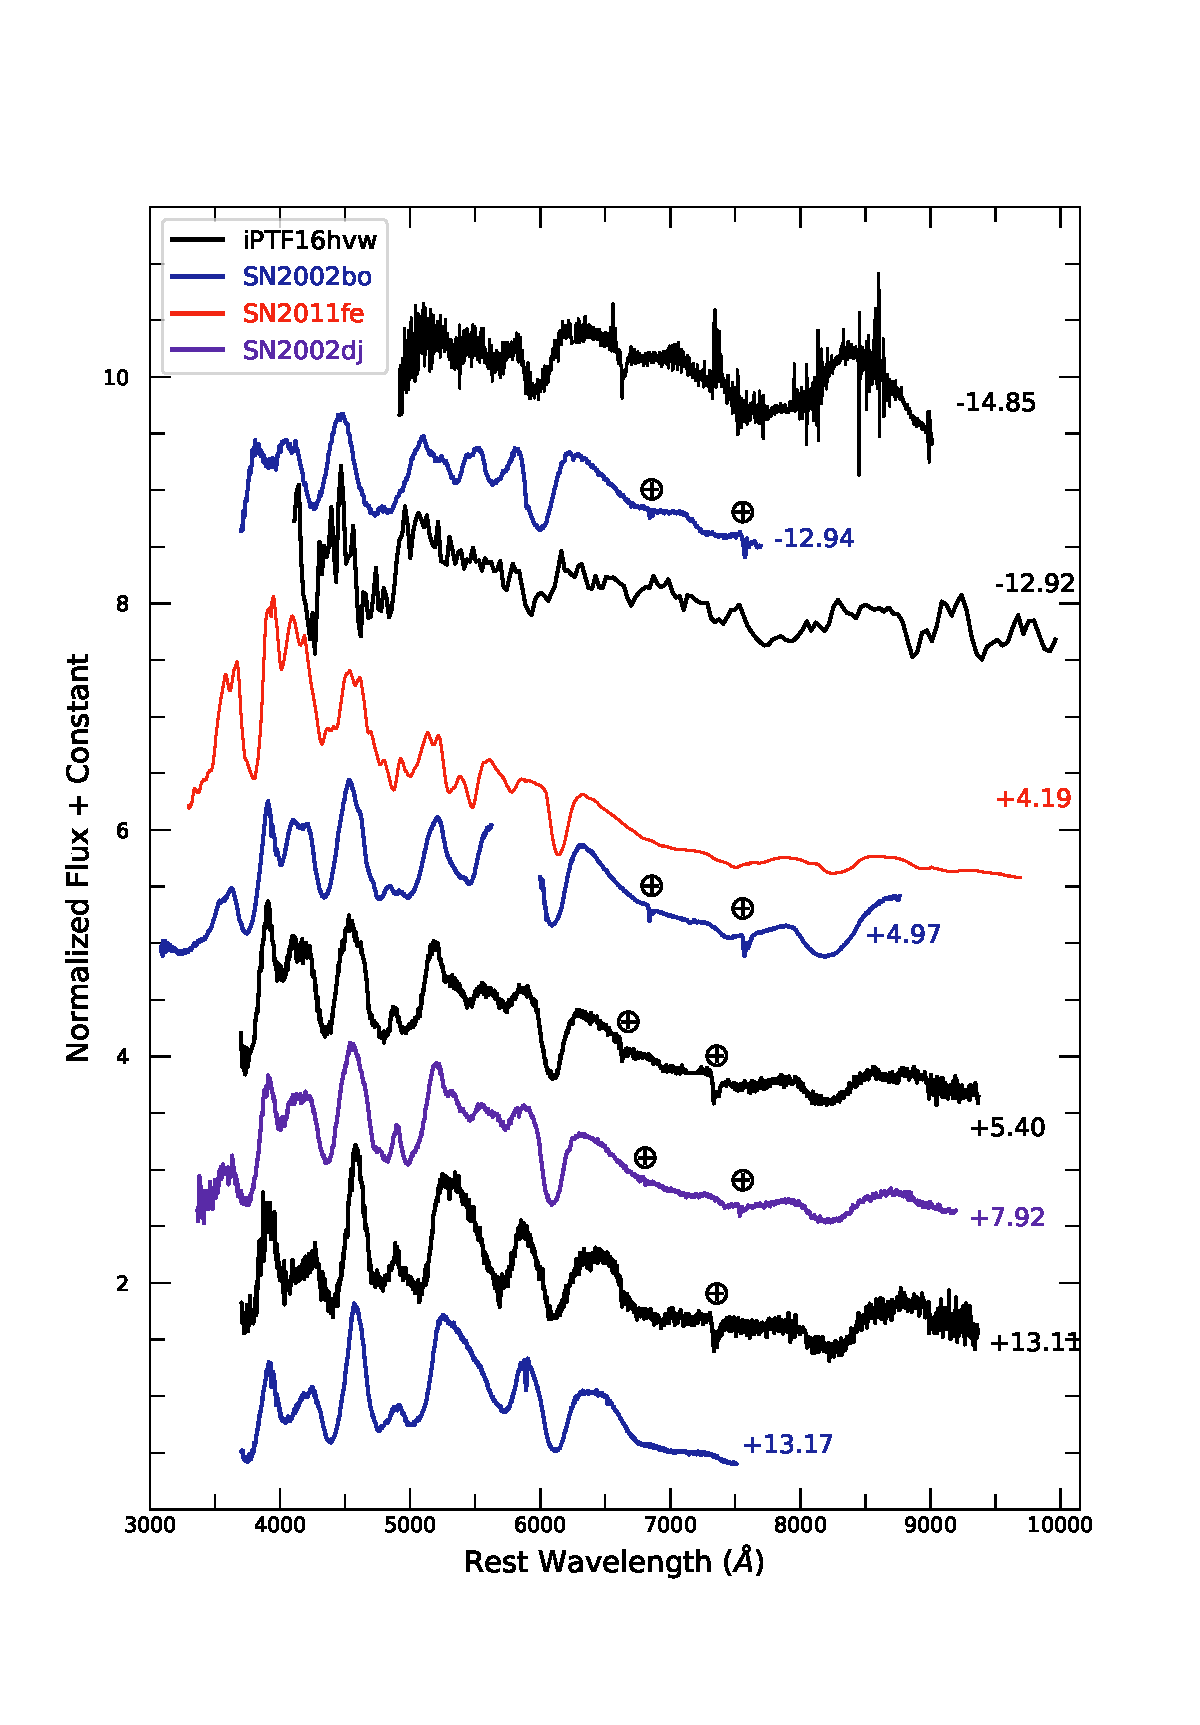
\includegraphics[width=80mm, height=120mm]{figure1.pdf}
% \caption{Spectral evolution....}
% \end{figure}

\section{Photometry}
Photometry ranging from -13 to +30 days were obtained for iPTF16hvw in the SDSS u, g, r and i bands. We used the sncosmo software package to generate simulated photometric data for SN2011fe in the SDSS u, g, r and i bands, and used this data to compare iPTF16hvw and SN2011fe color evolution. We also fit the P60 light curves using the SALT2 template (Guy et al. 2007). Because SALT2 performs poorly at early times, we excluded observations at phases below -10 d. The SALT2 fit reports the time of rest-frame B-band maximum to be MJDmax = 57,714.380 $\pm$ 0.060, the coefficient of the zeroth principle component $x_{0}$ = 0.001793 $\pm$ .000026, the coefficient of the first principle component $x_{1}$ = 0.07 $\pm$ 0.11, and the color term c = 0.2122 $\pm$  0.0095. 
We modeled the early light curve as a power law,
\begin{equation}
f(t) = \left\{
        \begin{array}{ll}
            a+ b(t - t_{0})^{\alpha}& \quad t  \geq t_{0} \\
            a & \quad t < t_{0}
        \end{array}
    \right.
\end{equation}

where $t_{0}$ is the time of first light, $\alpha$ is the power law index, and $t$ is the time measured in the SN restframe.  Assuming Gaussian uncertainties between the data and model, we used the software package emcee to sample the posterior parameter space for the best fit $t_{0}$  and $\alpha$ parameters in both the g and R bands. We have reason to believe (include specifics) the flux uncertainties are undervalued, so we also included an additional uncertainty parameter in the likelihood. We used wide, flat priors on all of the parameters. Unfortunately, the limited amount of early photometric data we have at our disposal led to a degeneracy between $t_{0}$ , $\alpha$ , and b, and the inability to constrain the b parameter. Despite extremely high b values and b values extremely close to 0 being unlikely, the sampler searched posterior values for b ranging from 0 to 750.  Without the ability to constrain b, we are unable to properly constrain $t_{0}$  or  $\alpha$. However, emcee still allows us to marginalize $t_{0}$ and $\alpha$ over the distributions of the other parameters. Marginalization gave us values for  $t_{0}$ and $\alpha$ of (put values here).
\end{document}
